\newcommand{\colA}[1]{\begin{columns}[t]\begin{column}{#1}} 
\newcommand{\colB}[1]{\end{column}\begin{column}{#1}} 
\newcommand{\colEnd}{\end{column}\end{columns}}

\usetheme{Warsaw}
\usecolortheme{seahorse}
% keine Navigationspfeile
\setbeamertemplate{navigation symbols}{} % keine Navigations-Buttons
\graphicspath{{/home/jogi/work/CalliopeMini-ProgrammierenLernen/}}
% Fußzeile mit Titel und Seitenr.
\definecolor{mygray}{gray}{0.75}
\setbeamertemplate{footline}{{\vspace{2mm}\color{mygray}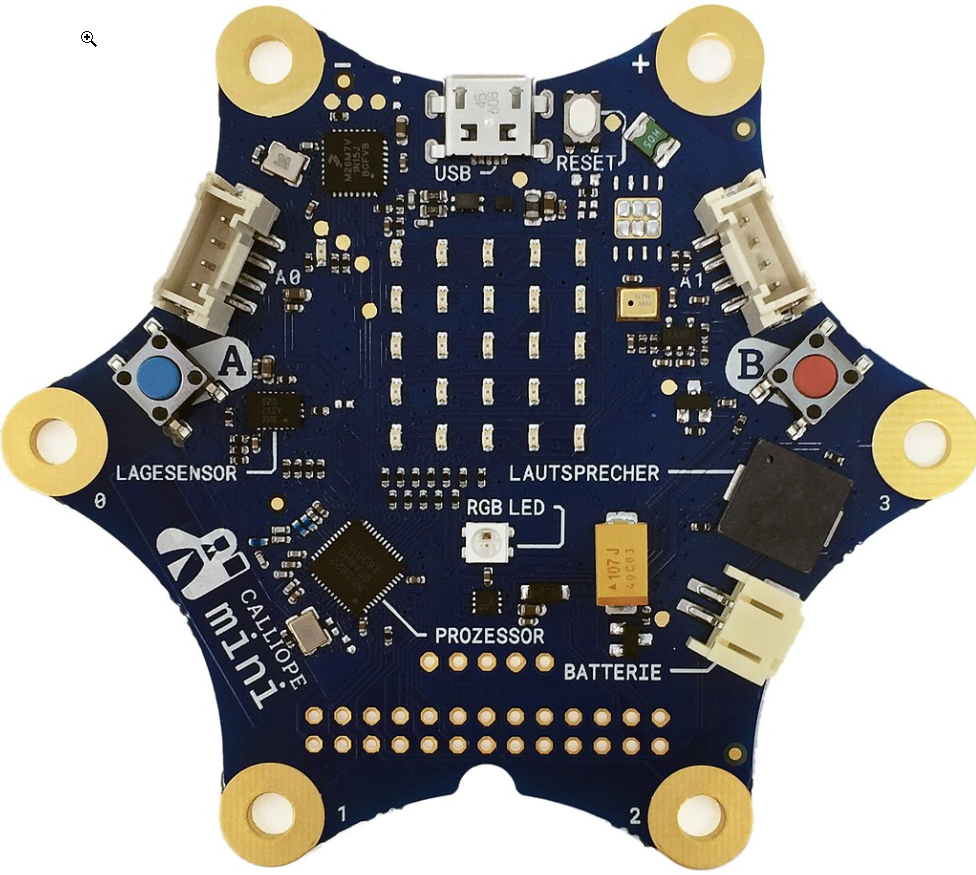
\includegraphics[width=20pt]{./calliope.png}\hspace*{2mm}\tiny\inserttitle\hspace*{80pt}\hfill
\includegraphics[width=20pt]{turbine.png}\insertframenumber/\inserttotalframenumber\ \hspace*{2mm}\vspace{2mm}}}

% Schrift für URLs
\definecolor{myblue}{rgb}{0.2 0.0 0.8}
\renewcommand{\UrlFont}{\color{myblue}\footnotesize\sf}

% Schriftgröße Listings
\RequirePackage{fancyvrb}
\DefineVerbatimEnvironment{Highlighting}{Verbatim}%
  {commandchars=\\\{\},fontsize=\footnotesize} 
\DefineVerbatimEnvironment{Verbatim}{Verbatim}%
  {fontsize=\footnotesize}

%%% Local Variables: 
%%% mode: latex
%%% TeX-master: t
%%% End: 
